
\documentclass{article}
\LARGE
% Language setting
% Replace `english' with e.g. `spanish' to change the document language
\usepackage[english]{babel}

% Set page size and margins
% Replace `letterpaper' with `a4paper' for UK/EU standard size
\usepackage[letterpaper,top=2cm,bottom=2cm,left=3cm,right=3cm,marginparwidth=1.75cm]{geometry}


\usepackage{tikz}
\usetikzlibrary{shapes.geometric, arrows}
\tikzstyle{startstop} = [rectangle, rounded corners, minimum width=3cm, minimum height=1cm,text centered, draw=black, fill=red!30]
\tikzstyle{io} = [trapezium, trapezium left angle=70, trapezium right angle=110, minimum width=3cm, minimum height=1cm, text centered, draw=black, fill=blue!30]
\tikzstyle{process} = [rectangle, minimum width=3cm, minimum height=1cm, text centered, draw=black, fill=orange!30]
\tikzstyle{decision} = [diamond, minimum width=3cm, minimum height=1cm, text centered, draw=black, fill=green!30]
\tikzstyle{arrow} = [thick,->,>=stealth]




\pgfdeclarelayer{bg}
\pgfsetlayers{bg,main}

% Useful packages
\usepackage{amsmath}
\usepackage{amsfonts}
\usepackage{graphicx}
\usepackage{float}
\usepackage[colorlinks=true, allcolors=cyan]{hyperref}
%\numberwithin{equation}{subsection}
\usepackage{graphicx,wrapfig,lipsum,subfigure,sidecap,epsfig}
\usepackage{caption}
\usepackage{cancel}
%\usepackage{graphicx,subfigure,sidecap,epsfig} % Rouslan's subfig package
\usepackage{soul}
%\usepackage[colorlinks=true,linkcolor=red]{hyperref}%

\graphicspath{{figures/}}


%%% Todos
\newcommand{\todo}[1]{\vspace{5 mm}\par \noindent
\marginpar{\textsc{\tiny \hspace{0.5cm} ToDo}} \framebox{\begin{minipage}[c]{0.95
\textwidth} \small \tt #1 \end{minipage}}\vspace{5 mm}\par}



\title{MATH 102 Linear algebra practice problems}
\author{Rauan}

\begin{document}
\maketitle

\begin{abstract}
  Practice problems from labs (Anton-Rorres). 
\end{abstract}

\tableofcontents

\section{Lab 1} \label{sec:Lab-1}
\begin{enumerate}
\item 3.1.18. Let $\mathbf{u}=(2,1,0,1,-1)$ and $\mathbf{v}=(-2,3,1,0,2)$. Find scalars $a$ and $b$ so that $a \mathbf{u}+b \mathbf{v}=(-8,8,3,-1,7)$.

\textbf{Solution:} We have two unknowns and 5 equations. Let us check zero entries. vector $\mathbf{u}$ has zero in third entry $u_3$, hence $(a)(u_3)+(b)(v_3)=(b)(1)=3$. Repeat for the 4th entry of $\mathbf{v}$, we get $a=-1$. Surprisingly $-\mathbf{u}+3\mathbf{v}$ add up to the desired result.

\item 3.1.21. Show that there do not exist scalars $c_1, c_2$, and $c_3$ such that
$$
c_1(-2,9,6)+c_2(-3,2,1)+c_3(1,7,5)=(0,5,4)
$$

\textbf{Solution:}

The given equation can be written as a system of linear equations:
$$
\begin{aligned}
-2 c_1-3 c_2+c_3 & =0 \\
9 c_1+2 c_2+7 c_3 & =5 \\
6 c_1+c_2+5 c_3 & =4
\end{aligned}
$$
We can solve this system by substitution or elimination, but to avoid too many computations, let's observe the first equation. It tells us that $c_3=2 c_1+3 c_2$.
Substitute $c_3$ into the second and third equations:
$$
\begin{gathered}
9 c_1+2 c_2+7\left(2 c_1+3 c_2\right)=5 \\
6 c_1+c_2+5\left(2 c_1+3 c_2\right)=4
\end{gathered}
$$
Simplify to get:
$$
\begin{aligned}
& 23 c_1+23 c_2=5 \\
& 16 c_1+16 c_2=4
\end{aligned}
$$
Divide the first equation by 23 and the second by 16 :
$$
\begin{aligned}
& c_1+c_2=\frac{5}{23} \\
& c_1+c_2=\frac{4}{16}=\frac{1}{4}
\end{aligned}
$$
We see that the two equations are contradictory $\left(\frac{5}{23} \neq \frac{1}{4}\right)$, so there are no solutions for $c_1, c_2$, and $c_3$. Therefore, it's not possible to express the vector $(0,5,4)$ as a linear combination of the vectors $(-2,9,6)$, $(-3,2,1)$, and $(1,7,5)$.

\item 3.1.23. Let $P$ be the point $(2,3,-2)$ and $Q$ the point $(7,-4,1)$.
(a) Find the midpoint of the line segment connecting the points $P$ and $Q$.
(b) Find the point on the line segment connecting the points $P$ and $Q$ that is $\frac{3}{4}$ of the way from $P$ to $Q$.

  \textbf{Solution:}
  (a) The midpoint of a line segment connecting two points $P\left(x_1, y_1, z_1\right)$ and $Q\left(x_2, y_2, z_2\right)$ in threedimensional space is given by the point $M\left(\frac{x_1+x_2}{2}, \frac{y_1+y_2}{2}, \frac{z_1+z_2}{2}\right)$.
Substituting the given coordinates of points $P(2,3,-2)$ and $Q(7,-4,1)$ into the formula, we get the midpoint as:
$$
M\left(\frac{2+7}{2}, \frac{3+(-4)}{2}, \frac{-2+1}{2}\right)=M\left(\frac{9}{2}, \frac{-1}{2}, \frac{-1}{2}\right)=M(4.5,-0.5,-0.5)
$$
(b) The point that is $\frac{3}{4}$ of the way from $P$ to $Q$ can be found using the formula $R=P+t(Q-P)$, where $t$ is the fraction of the distance from $P$ to $Q$.
Substituting $t=\frac{3}{4}$ and the coordinates of points $P(2,3,-2)$ and $Q(7,-4,1)$ into the formula, we get:
$$
R=P+t(Q-P)=(2,3,-2)+\frac{3}{4}[(7,-4,1)-(2,3,-2)]=(2,3,-2)+\frac{3}{4}(5,-7,3)
$$
Solving this gives us:
$$
R=(2,3,-2)+(3.75,-5.25,2.25)=(5.75,-2.25,0.25)
$$
So the point that is $\frac{3}{4}$ of the way from $P$ to $Q$ is $(5.75,-2.25,0.25)$.

\item 3.1.28. If the sum of three vectors in $R^3$ is zero, must they lie in the same plane? Explain.

\textbf{Solution:} Let's denote the three vectors as $\mathbf{a}, \mathbf{b}$, and $\mathbf{c}$. If their sum is zero, we have $\mathbf{a}+\mathbf{b}+\mathbf{c}=\overrightarrow{0}$.
This equation can be rewritten as $\mathbf{c}=-\mathbf{a}-\mathbf{b}$.
This shows that vector $\mathbf{c}$ can be expressed as a linear combination of vectors $\mathbf{a}$ and $\mathbf{b}$. In other words, $\mathbf{c}$ lies in the plane spanned by $\mathbf{a}$ and $\mathbf{b}$.

Therefore, all three vectors $\mathbf{a}, \mathbf{b}$, and $\mathbf{c}$ lie in the same plane. This holds true for any three vectors in $R^3$ whose sum is zero.

\item 3.2.1-2. In Exercises 1-2, find the norm of $\mathbf{v}$, and a unit vector that is oppositely directed to $\mathbf{v}$.
1. (a) $\mathbf{v}=(2,2,2)$
(b) $\mathbf{v}=(1,0,2,1,3)$
2. (a) $\mathbf{v}=(1,-1,2)$
(b) $\mathbf{v}=(-2,3,3,-1)$
\end{enumerate}

\subsection{Online quiz related:}



\begin{enumerate}
  \item[1.]  In $\mathbb{R}^2$, you are given the points $A(-17,-13)$ and $X(17,7)$. Find $t$ such that the point $C\left(-\frac{68}{5}, t\right)$ lies on the line through $A$ and $X$. Answer (use a ratio, not a decimal): $t=$

\textbf{Solution:} 

If we have $(-17,-13)+p(34,20)=\left(-\frac{68}{5}, t\right)$, then from the first coordinate we get $-17+34 p=-\frac{68}{5}$, which simplifies to $170 p=17$, and hence $p=\frac{1}{10}$.

Plugging this into the second coordinate gives us $-13+\frac{1}{10} \cdot 20=t$, which simplifies to $-13+2=t$, hence $t=-11$.
So, the point $C$ that lies on the line through $A$ and $X$ is indeed $C\left(-\frac{68}{5},-11\right)$.
  \item[2.] Given a vector $\mathbf{v}=(x_{0}, y_{0}, z_{0})\in \mathbb{R}^3$. It gets reflected against $xy$ plane and then subsequently reflected against $yz$ plane. Find the resultant reflection. 

  \textbf{Solution:}

  When a vector is reflected against a plane, the component of the vector perpendicular to the plane changes sign, while the components parallel to the plane remain unchanged.
\begin{enumerate}
  \item  Reflecting $\mathbf{v}=\left(x_0, y_0, z_0\right)$ against the $x y$ plane means the $z$-component changes sign, resulting in a new vector $\mathbf{v}_r=\left(x_0, y_0,-z_0\right)$.
  \item Reflecting $\mathbf{v}_r$ against the $y z$ plane means the $x$-component changes sign, resulting in a new vector $\mathbf{v}_{rr}=\left(-x_0, y_0,-z_0\right)$.

\end{enumerate}
 
  So, the resultant reflection of $\mathbf{v}$ against the $x y$ plane followed by the $y z$ plane is $\mathbf{v}_{rr}=\left(-x_0, y_0,-z_0\right)$.

\end{enumerate}

\subsection{Assignment related:} 

1. (b) Describe the span of each of the following sets.
$$
A=\{(2,-1),(1,5)\} \quad B=\{(2,-1),(6,-3)\}
$$
Two linearly Independent vectors span plane. Two dependent - span a line. 

1. (c) Let $\mathbf{v}_{\mathbf{1}}=(0,0,1,-1)$ and $\mathbf{v}_{\mathbf{2}}=(3,2,-1,1)$ and $\mathbf{v}_{\mathbf{3}}=(-1,0,2,-1)$.

i. Express $\mathbf{p}=(4,4,1,1)$ as a linear combination of the vectors $\mathbf{v}_{\mathbf{1}}, \mathbf{v}_{\mathbf{2}}, \mathbf{v}_{\mathbf{3}}$. \textbf{Solution} is similar to to 3.1.18 at the beginning of this lab. 

ii. Show that $\mathbf{q}=(1,3,3,-2)$ does not belong to the span of $\left\{\mathbf{v}_{\mathbf{1}}, \mathbf{v}_{\mathbf{2}}, \mathbf{v}_{\mathbf{3}}\right\}$. \textbf{Solution} is similar to 3.1.21 from the beginning of this lab, i.e. "Does not belong to the span" is same as $c_{1},c_{2},c_{3}$ do not exist.  

\section{Lab 2}\label{sec:lab2}

The $n$-th roots of a complex number $z=r e^{i \varphi}$ are
$$
\alpha_k=\sqrt[n]{r} e^{i \frac{\varphi}{n}+i \frac{2 \pi}{n} k} \quad \text { where } k \in\{0,1, \ldots, n-1\},
$$
since
$$
\alpha_k^n=r e^{i \varphi+i 2 \pi k}=r e^{i \varphi} .
$$

Exercises:
\begin{enumerate}
\item In each of the following, determine the indicated roots of the given complex number. When it is possible, write the roots in the form a $\mathrm{C}$ bi , where a andb are real numbers and do not involve the use of a trigonometric function. Otherwise, leave the roots in polar form.

\begin{enumerate}
\item The two square roots of $16 i$.
\item The two square roots of $2+2 i \sqrt{3}$.
\item The three cube roots of $5\left(\cos \left(\frac{3 \pi}{4}\right)+i \sin \left(\frac{3 \pi}{4}\right)\right)$.
\item The five fifth roots of unity.
\item The four fourth roots of $\left(\frac{1}{2}-\frac{\sqrt{3}}{2} i\right)$.
\item The three cube roots of $1+\sqrt{3} i$.
\end{enumerate}
\textbf{Solution}:
\begin{enumerate}
  \item[(a)] Write $16 i=16\left(\cos \left(\frac{\pi}{2}\right)+i \sin \left(\frac{\pi}{2}\right)\right)$. The two square roots of $16 i$ are
$$
\begin{gathered}
4\left(\cos \left(\frac{\pi}{4}\right)+i \sin \left(\frac{\pi}{4}\right)\right)=2 \sqrt{2}+2 i \sqrt{2} \\
4\left(\cos \left(\frac{5 \pi}{4}\right)+i \sin \left(\frac{5 \pi}{4}\right)\right)=-2 \sqrt{2}-2 i \sqrt{2}
\end{gathered}
$$

  \item[(c)] The three cube roots of $5\left(\cos \left(\frac{3 \pi}{4}\right)+i \sin \left(\frac{3 \pi}{4}\right)\right)$ are
$$
\begin{gathered}
\sqrt[3]{5}\left(\cos \left(\frac{\pi}{4}\right)+i \sin \left(\frac{\pi}{4}\right)\right)=\sqrt[3]{5}\left(\frac{\sqrt{2}}{2}+\frac{\sqrt{2}}{2} i\right) \\
\sqrt[3]{5}\left(\cos \left(\frac{11 \pi}{12}\right)+i \sin \left(\frac{11 \pi}{12}\right)\right) \\
\sqrt[3]{5}\left(\cos \left(\frac{19 \pi}{12}\right)+i \sin \left(\frac{19 \pi}{12}\right)\right)
\end{gathered}
$$
\end{enumerate}




\item Use DeMoivre's Theorem to determine each of the following powers of a complex number. Write the answer in the form $a+b i$, where $a$ and $b$ are real numbers and do not involve the use of a trigonometric function.
\begin{enumerate}
\item $(2+2 i)^6$
\item $(\sqrt{3}+i)^8$ 
\item $\left(\frac{1}{2}+\frac{\sqrt{3}}{2} i\right)^3$ 
\item $2\left(\cos \left(\frac{\pi}{15}\right)+i \sin \left(\frac{\pi}{15}\right)\right)^{10}$ 
\item $(1+i \sqrt{3})^{-4}$ 
\item $(-3+3 i)^{-3}$
\end{enumerate}

\textbf{Solutions:}
  \begin{enumerate}
    \item[(a)] $(2+2 i)^6=\left[\sqrt{8}\left(\cos \left(\frac{\pi}{4}\right)+i \sin \left(\frac{\pi}{4}\right)\right)\right]^6=512 i$
    \item[(b)] $(\sqrt{3}+i)^8=\left[2\left(\cos \left(\frac{\pi}{6}\right)+i \sin \left(\frac{\pi}{6}\right)\right)\right]^8=-128-128 \sqrt{3} i$
  \end{enumerate}
\end{enumerate}


\subsection{Online Quiz related}

Problems are trivial, some useful identities to use:
\begin{enumerate}
  \item $z = a+bi$.
  \item $\bar{z}=a-bi$ is called complex conjugate of $z$.
  \item $z\bar{z}=a^2+b^2$.
  \item $z^{-1}z=1$, hence $z=a+bi\implies {z}^{-1}=\frac{1}{a+bi}$. Where $z^{-1}$  is called inverse of $z$.
  \item To convert a fractional complex number $z=\frac{c+di}{e+fi}$ to a standard form $z=a+bi$ multiply both numerator and denominator of $z$ by complex conjugate of denominator, i.e. $z=\frac{c+di}{e+fi}\frac{e-fi}{e-fi}$. Now denominator is real number, need to simplify the numerator a bit.
\end{enumerate}

With vectors. Two vectors $\vec{v},\vec{u}$ are parallel to each other if and only if (iff) $\exists c\in \mathbb{R}: \vec{v}=c\vec{u}$. (exists some real number $c$ such that $\vec{v}$ is a scaled version of $\vec{u}$), For non-parallel use negation of the statement - vectors $\vec{u},\vec{v}$ are not parallel iff there exists no $c$ such that $\vec{u}=c\vec{v}$.

Sum of two non-parallel vectors (excl. zero) produces a third non-parallel vector. 

\subsection{Assignment related}

\begin{enumerate}
  \item[2.]
  \begin{enumerate}
    \item [a,b.] trivial
    \item[c.] We consider the movement of the particles in this problem. Hence, time is common for both equations of the line. Need to minimize the distance - apply Pythagorian theorem for three coordinates between two lines, then use your OP skills from Calculus 1 to find that bottom tip of parabola.
    \item[d.] Trivial. Collide $\iff$ ${l}_1(t)={l}_2(t)$ for some $t$
    \item[e.] Trivial. Path intersection means lines are time independent. Use two different time variables $t,s$ for each line separately and try to find these $t,s$. 
  \end{enumerate}
  \item[3.] Trivial. To represent the complex number in the polar form multiply and divide by its magnitude. One magnitude becomes the $r$, another together with the number itself becomes normalized and can be expressed as an exponent. 
   
  
  ($z=re^{i\theta}=r(\cos\theta+i\sin\theta) =-r(-\cos\theta+i[-\sin\theta])= -r(\cos(\theta+\pi) + i\sin(\theta+\pi))$, by the same logic can we make radius a complex number with $i\phi$ argument and shift exponential part by angle $\phi$, definition of exponential form needs clarification.)
\end{enumerate}

\section{Lab 3}
\subsection{Online Quiz related}
\begin{enumerate}
\item For a fixed complex number $w$ consider the complex linear transformation
$$
L: \mathbb{C} \longrightarrow \mathbb{C}, \quad L(z)=w \cdot z
$$
What is $w$ if $L$ scales $\mathbb{C}$ by the factor $12$ while rotating $\mathbb{C}$ clockwise through the angle
$$
\theta=\frac{\pi}{3}
$$

\textbf{Solution:} Given our linear transformation $L$ is a product of two elements in $\mathbb{C}$ we can use the property of polar forms. When two complex numbers get multiplied in polar forms the result is the product of their radii and exponent of sum of their angles. 
\item With the complex numbers
\begin{itemize}
\item $a=6-7 \cdot \mathrm{i}$
\item $w=\mathrm{i}-3$
\item $z=\mathrm{i}+2$
\end{itemize}
Compute $a(\bar{w}-z)^2+a(w+\bar{z})^2=$

  \textbf{Solution:} Have to compute honestly. Note that $w,z$ are written in non-standard format, it is imaginary then real part, hence need to pay attention when taking complex conjugate ($z=Re(z) + Im(z); \bar{z}= Re(z) - Im(z)$).
I am not honest, used Matlab:
\begin{verbatim} 
>>a = 6-7*i; w = i - 3; z = i + 2; a*(conj(w)-z)^2 + a*(w+conj(z))^2;
ans = 272 - 34i 
\end{verbatim}
  \item Find a complex number 𝑤 such that  $u^{20}=−1$.

  \textbf{Solution:} We know how to take an $n^{th}$ root (Section~\ref{sec:lab2}). Convert to polar then divide by $n$. In this case any of 20 roots should be sufficient.
  \item $\text { Find a complex number } w \text { such that } w^{48}=e^{\pi i / 63}$ Similar to above. 
  \item For an integer $n \geq 1$, recall that an $n$-th root of unity is any complex number $\omega$ such that
$$
\omega^n=1
$$
Certainly, $\omega=1$ is an $n$-th root of unity for every $n$. Now, if $n=22$, then an $n$-th root of unity which is distinct from 1 is.

\textbf{Solution:} Add any $2\pi k; k\neq 0$ to your $w=1$ and then divide by $22$.

\item Find 3 distinct 46-th roots of unity. 

\textbf{Solution:} Recall unity, $w=1$ add any three non-zero multiples of $2\pi$ then divide by 46. 

\item Consider the polynomial
$$
p(z)=z^3+14 z^2+82 z+272
$$
Factor $p$ over the complex numbers, using the information that $\zeta_1=-8$ is a root of $p$. 

\textbf{Solution:} Perform column division (long division, polynomial division).  
\begin{figure}[H]
\centering
  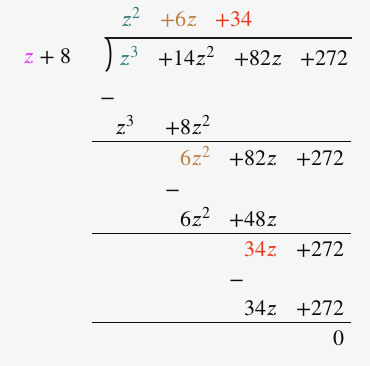
\includegraphics[scale=0.35]{lab3polynomial.png}
  \caption{Long division.}
\end{figure}

Then factor the result using your favourite method. 

$z^2+6z+34=z^2+2(z)(3) + 3^2 - 3^2 + 34=(z+3)^2-9+34=(z+3)^2+25=(z+3)^2+5^2=(z+3)^2-(5i)^2=(z+3-5i)(z+3+5i)$

\item Consider the polynomial
$$
p(z)=z^4+12 z^3+57 z^2+132 z+136
$$
Factor $p$ over the complex numbers, using the information that $\zeta_1=-2+2 i$ is a root of $p$.

\textbf{Solution:} Since coefficients for $p$ are all real numbers then the complex conjugate of $\zeta_1$ is also a root. Means $\zeta_2=-2-2i$. Then $(z-\zeta_1)(z-\zeta_2)=(z+2-2i)(z+2-2i)$. 

\begin{verbatim}
	>> syms z; simplify((z+2-2*i)*(z+2+2*i))
ans =
z^2 + 4*z + 8
\end{verbatim}

Perform corner division.

\begin{figure}[H]
\centering
  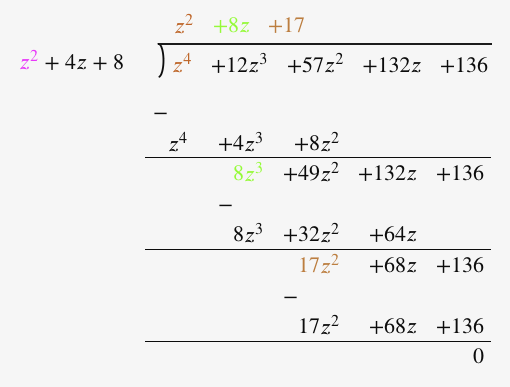
\includegraphics[scale=0.35]{lab3polynomialBIG.png}
  \caption{Long division.}
\end{figure}

Factor the result using your favourite method. $z^2+8z+17=z^2+2(z)(4) + 4^2 - 4^2 + 17 = (z+4)^2-16+17=(z+4)^2 + 1 = (z+4)^2 -(i)^2=(z+4-i)(z+4+i)$. Thus, we find $\zeta_3,\zeta_4.$

\item Dot product question is trivial. 

\textbf{Solution:} Use definition $u\cdot v = \| u \| \| v \| \cos(\widehat{uv})$, where $\| .\|$ is length. 

\item  An orthogonal set of vectors is a set of vectors in which every pair of vectors within the set are orthogonal to each other.
Among the sets of vectors listed below, identify the orthogonal ones. - Type ' 1 ' for 'orthogonal set', and type ' 0 ' for 'not orthogonal set'
$$
\begin{aligned}
& (-3,-3,-10,-40,-16),(10,-16,3,0,3),(33,-26,10,0,8) \\
& (21,53,-28,-20,1),(18,14,12,55,316),(0,-1300,-3195,1028,0) \\
& (-3,-10),(-10,3),(3,10) \\
& (53,12,1),(-40,26,1808),(21670,-95864,1858) \\
& (-8,1,-16),(12,320,14),(5134,-80,-2572),(-20,12,-8)
\end{aligned}
$$

\textbf{Solution:} Use dot product property - the dot product of perpendicular vectors means $\cos(\theta)=\cos(90^\circ)=0$, hence their dot product is zero. (Since it is online quiz you might want to use a calculator).

\end{enumerate}

\bibliographystyle{plain}
\bibliography{Zotero}

\appendix

\section{Appendix}


\end{document}

